\section{Scan Conversion}

Scan conversion (also called rasterization) is the problem of converting our objects to the discrete pixel space, e.g. deciding which pixel lie inside our object. 


\subsection{Scan Conversion of Lines}

\textbf{Bresenham lines} choose the closest pixel at each intersection. The goal is to have a fast decision which pixel has to be drawn next. It does this by using the position of the midpoint $m$ with respect to the intersection point $q$ as a criterion.
\begin{center}
	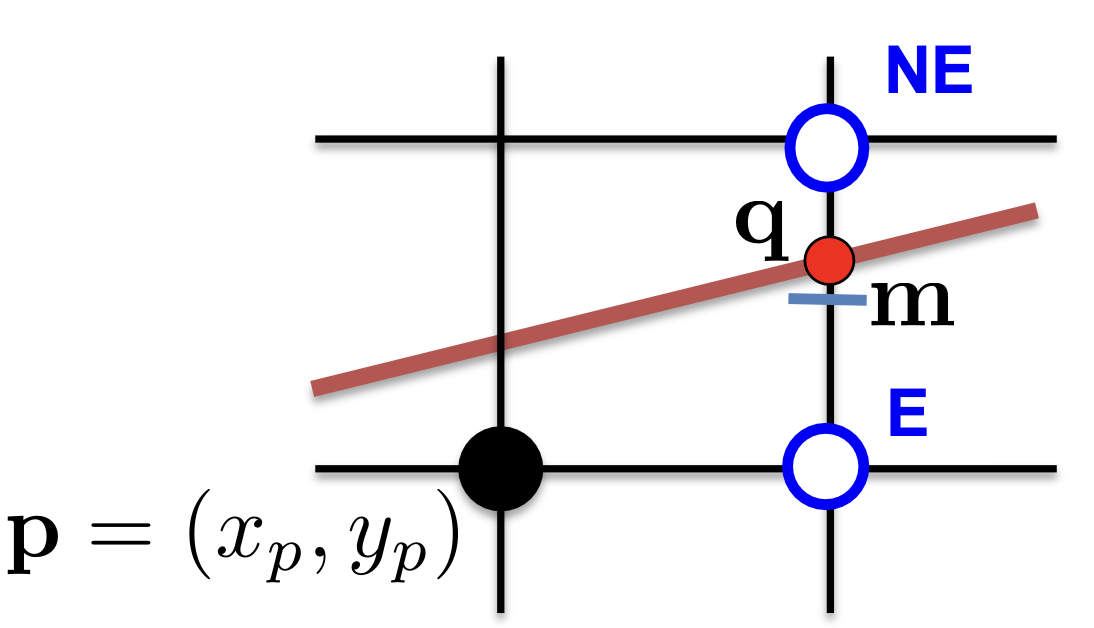
\includegraphics[width=0.7\linewidth]{bresenham.png}
\end{center}

Given $f(x,y) = ax + by + c = 0$ as the implicit equation of the straight line, it decides based on $d = f(m)$. If $d < 0$ select pixel E, else select pixel NE. After the first decision, we can base our update criterion based on the choice E or NE.
$$\text{Pixel NE : } d_{new} = d_{old} + \Delta y - \Delta x$$
$$\text{Pixel E : } d_{new} = d_{old} + \Delta y$$

\subsection{Scan Conversion of Polygons}

Filled polygons (especially triangles) are the most important graphics primitives. The straightforward solution would be to perform an inside test for each pixel, but this is very inefficient. Instead we process scan line after scan line. We call a group of picked pixels inside a scan line a \textbf{span}. The algorithm then works as follows:
\begin{enumerate}
	\item Calculate all intersections of the scan line
	\item Sort the intersection points by ascending x-coordinates
	\item Fill all spans in between two consecutive intersection points if the parity is odd
\end{enumerate}

\begin{center}
	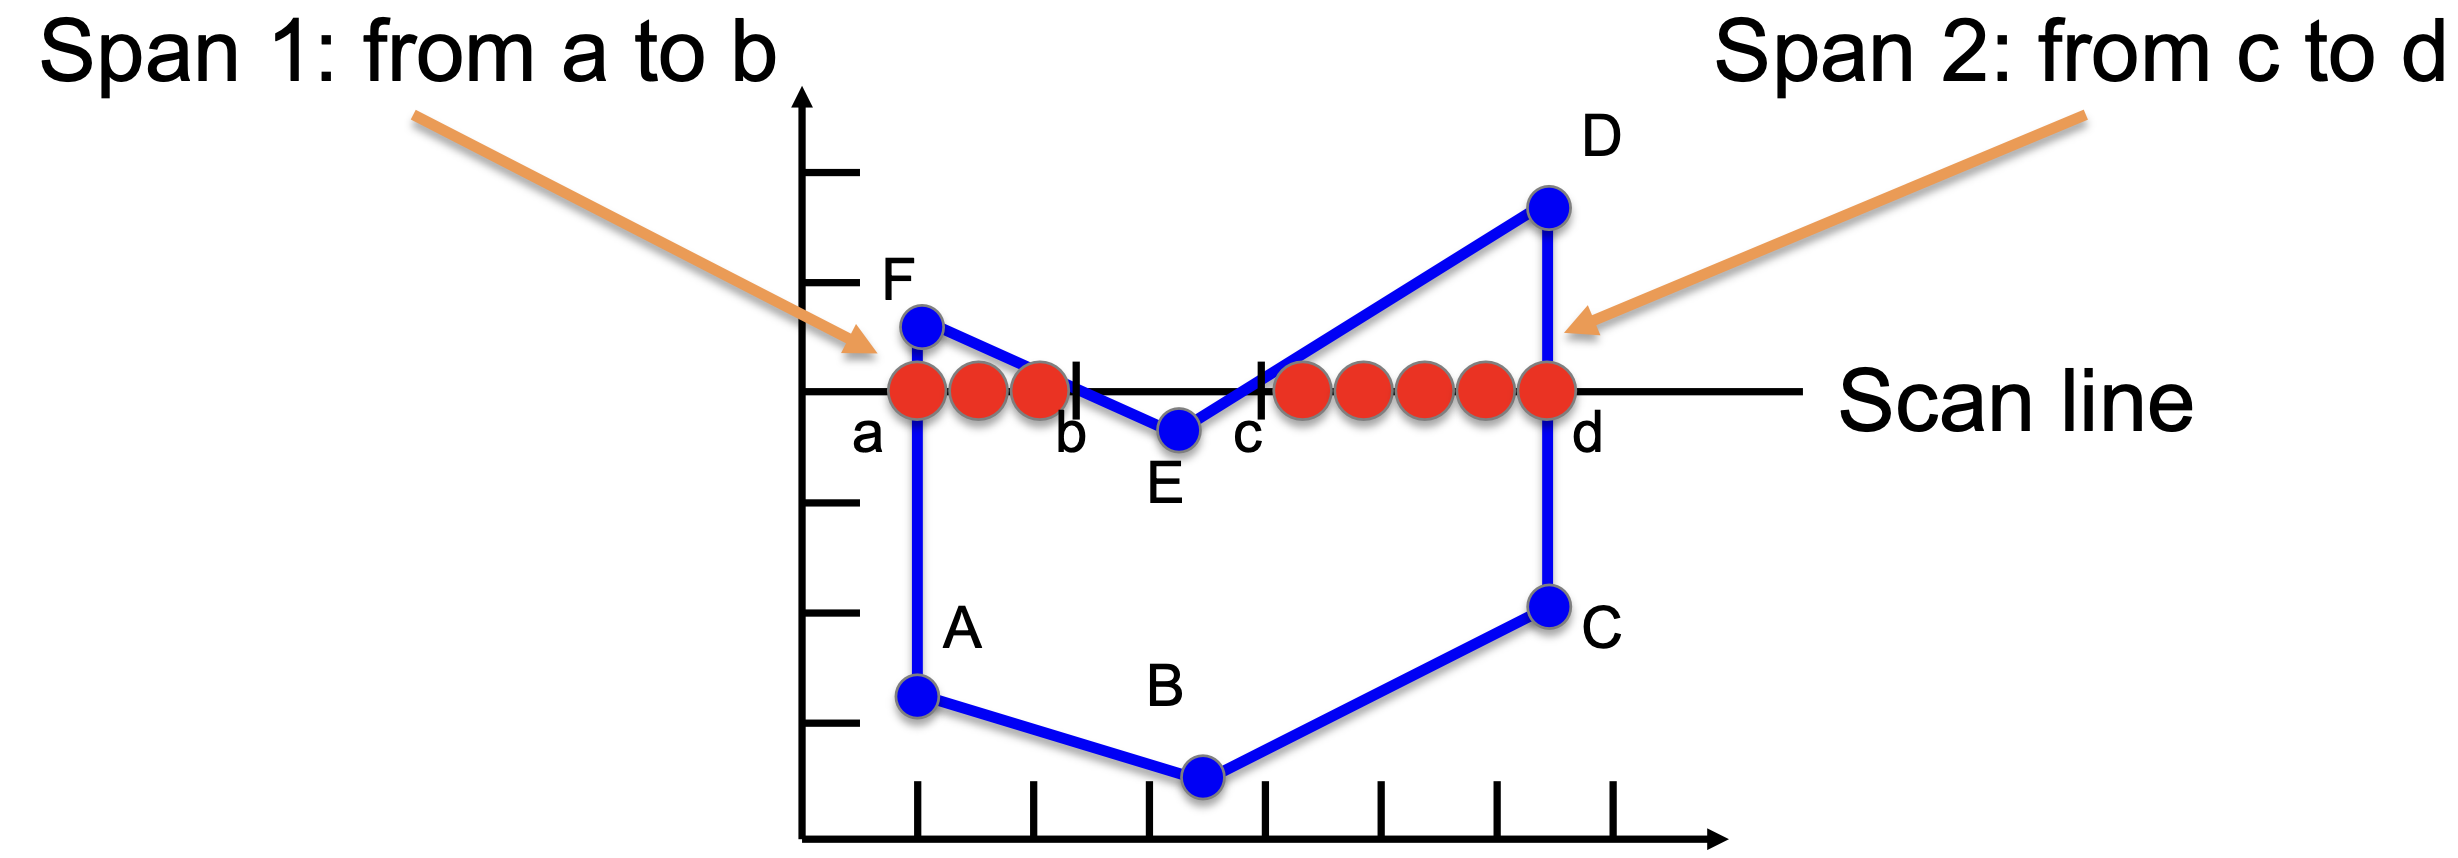
\includegraphics[width=0.9\linewidth]{scan_line.png}
\end{center}